% Metódy inžinierskej práce

\documentclass[10pt,twoside,slovak,a4paper]{article}

\usepackage[slovak]{babel}
%\usepackage[T1]{fontenc}
\usepackage[IL2]{fontenc} % lepšia sadzba písmena Ľ než v T1
\usepackage[utf8]{inputenc}
\usepackage{graphicx}
\usepackage{url} % príkaz \url na formátovanie URL
\usepackage{hyperref} % odkazy v texte budú aktívne (pri niektorých triedach dokumentov spôsobuje posun textu)

\usepackage{cite}
%\usepackage{times}

\pagestyle{headings}

\title{Efektivita a dopad dištančného vzdelávania na vyučovanie\thanks{Semestrálny projekt v predmete Metódy inžinierskej práce, ak. rok 2020/21, vedenie: Jozef Sitarčík}}

\author{Christian Danížek\\[2pt]
	{\small Slovenská technická univerzita v Bratislave}\\
	{\small Fakulta informatiky a informačných technológií}\\
	{\small \texttt{xdanizek@stuba.sk}}
	}

\date{\small 22. október 2020} % upravte

\begin{document}

\maketitle


\begin{abstract}
Vzdelávanie odjakživa prebiehalo výhradne prezenčne a  nebolo ani mysliteľné, aby prebiehalo iným spôsobom. Avšak s nástupom a vývojom technológií sa nám naskytuje nová alternatívna možnosť: dištančné vzdelávanie. Nový, dosiaľ neokresaný spôsob vyučovania so sebou prináša viacero výhod, ale aj nevýhod. Viacero vedcov a učiteľov vyjadrilo obavy o dôsledky vyučovania týmto novým spôsobom. V tomto článku sa teda budeme zaoberať základnou otázkou dištančného vzdelávania, a to efektívnosťou elektronického vzdelávania v porovnaní s klasickým spôsobom. Taktiež sa pozrieme na dôsledky príchodu dištančného vzdelávania na klasický spôsob vzdelávania.
\end{abstract}

\section{Úvod}
Dištančné vzdelávanie, aj napriek tomu, že je možné už dlhšie, je pre mnohých novinkou a platí to predovšetkým v čase pandémie súvisiacou s ochorením Covid-19. Až teraz, keď je takýto spôsob výučby často jediný možný, vidíme v plnej sile úskalia, ale aj výhody\cite{Zimmerman:Experiment}. Definície, s ktorými budeme pracovať v tomto článku sú vysvetlené v časti~\ref{definicie}. Základný problém, ktorý bol načrtnutý v úvode, a teda efektivita dištančného vzdelávania, bude vysvetlený v časti~\ref{efektivita}. V časti~\ref{dopad} bude vysvetlený dopad dištančného vzdelávania na klasický spôsob vzdelávania. Záverečné poznámky prináša časť~\ref{zaver}.

\section{Prezenčné a dištančné a vzdelávanie} \label{definicie}
\subsection{Prezenčné vzdelávanie}
Pod pojmom prezenčné vzdelávanie budeme rozumieť spôsob vzdelávania, v ktorom sú učiteľ a žiak v jednej miestnosti (poprípade nedaľeko od seba, ale fyzicky prítomní) a komunikácia prebieha medzi žiakom a učiteľom verbálnou a neverbálnou komunikáciou. V tomto článku budeme nazývať tento spôsob aj pod pojmom \textit{klasické vyučovanie} alebo tiež aj \textit{tradičné vyučovanie}.

\subsection{Dištančné vzdelávanie}
Pod pojmom dištančné vzdelávanie budeme rozumieť spôsob vzdelávania, kedy žiak a učiteľ nie su fyzicky prítomní pri sebe, ale sprostredkúvajú komunikáciu cez nejaké zariadenie. Môže ísť napríklad o počítač s mikrofónom a webkamerou. Komunikácia ale nemusí prebiehať naživo, vtedy ide o asynchrónne dištančné vzdelávanie. Populárne platformy pre videohovory v dnešnej dobe tvoria \textit{Microsoft Teams}, \textit{Cisco WebEx}, \textit{Google Meet} a ďalšie. V prípade asynchrónneho dištančného vzdelávania môže ísť napríklad o platformu \textit{Moodle}.

\section{Efektivita dištančného vzdelávania} \label{efektivita}
Pochopiť, ako efektívne je dištančné vzdelávania, je kľúčové pre budúci vývoj vzdelávania.

\subsection{Negatívne faktory}
Mohli by sme predpokladať, že s nástupom nových technológií sa bude dištančné vyučovanie využívať čoraz častejšie, poprípade úplne nahradí tradičné vyučovanie. Avšak, postupne si začíname uvedomovať, že prejsť na dištančné vzdelávanie nemusí byť dobrý nápad čo sa týka efektivity vzdelávania. Aj napriek tomu, že vieme používať technológie a poskytovať videohovor s desiatkami ľudí v reálnom čase, táto možnosť neposkytuje takú spätnú väzbu, skúsenosť, morálku a pozornosť ako tradičné vzdelávanie\cite{Wang:Investigation}\cite{Weidlich:Impact}.

\subsubsection{Technické problémy}
V prvom rade musíme samozrejme podotknúť, že efektivita dištančného vzdelávania môže byť značne negatívne ovplyvnená technickými problemámi alebo nemožnosťou študentov dovoliť si zariadenia pre dištančnú výučbu, prípade výpadkami telekomunikačných služieb (internetu). Percento študentov, ktorí budú mať podobné technické problémy, je malé, avšak každý študent by mal mať rovnaké podmienky na štúdium, a teda škola by mala zabezpečiť tieto možnosti pripojenia, ak ich študent potrebuje. To je však málokedy tak čo sa týka štátnych škôl.

Prípady môžu však byť aj iné. Môže taktiež ísť napríklad o prípad, kedy učiteľ nevie pracovať s platformou pre online vyučovanie, poprípade nie je technický zdatný celkovo. S takýmito prípadmi som sa osobne stretol veľakrát. V tomto prípade je negatívne ovplyvnené vzdelávanie celej skupiny.

\subsubsection{Psychologická otázka}
Hlavný negatívny faktor dištančného vyučovania je spojený s nedostatkom sociálneho kontaktu. Študenti môžu zažívať pocit úzkosti - že sú sami. Môžu trpieť nedostatkom motivácie. Komunikačná bariéra situáciu len zhoršuje. Tieto všetky negatívne faktory sa naplno ukazujú pri dlhodobom, výlučne dištančnom vzdelávaní.

\subsection{Pozitívne faktory}
\subsubsection{Pohodlie}
Najväčšou výhodou dištančného vyučovania je fakt, že poskytuje študentom vysoký stupeň pohodlia. Študenti sa môžu zúčastňovať vyučovania z pohodlia domova, alebo odkiaľkoľvek, kde sú na to vhodné podmienky, teda napríklad z práce. Študentom týmto spôsobom odpadáva nutnosť cestovať, čo môže mať veľkú výhodu pre študentov, ktorí nežijú blízko školy\cite{Weidlich:Impact}.

\subsection{Názory študentov a učiteľov} \label{nazory}
V štúdii z viacerých vysokých škôl v USA na prieskum efektívnosti dištančného vyučovania sa z 11 učiteľov 7 vyjadrilo, že tradičné vyučovanie je podľa nich efektívnejšie ako online vyučovanie a 4 učitelia sa vyjadrili, že online vyučovanie je efektívnejšie. Prekvapivo, ani jeden z učiteľov neuviedol, že by mali podla nich tieto dva spôsoby rovnakú efektivitu. 

Najzaujímavejšie sú ale výsledky od študentov, ktoré su zobrazené na obr. \ref{f:efektivitaStudenti}. Približne polovica študentov odpovedala, že sú podla nich výsledky vzdelávania približne rovnaké ako pri tradičnom vyučovaní. Až približne 42\% uviedlo, že tradičné vyučovanie má podľa nich lepšie výsledky. Len malé percento študentov uviedlo, že je online vyučovanie lepšie.\cite{Warren:Effectiveness}\cite{Balas:DistanceLearning}.

Čo sa týka porovnania náročnosti prezenčného a dištančného vyučovania, výsledky študentov a učiteľov sú zobrazené v tabuľke \ref{tab:narocnostStudentiUcitelia}. Až polovica študentov odpovedala, že dištančné vyučovanie je ťažšie, čo je pochopiteľné, pretože prinajmenšom treba čeliť komunikačnej prekážke. Učitelia odpovedali podobne, porovnateľne s možnosťou, že obtiažnosť je podľa nich rovnaká.

\begin{figure*}[h]
	\centering
	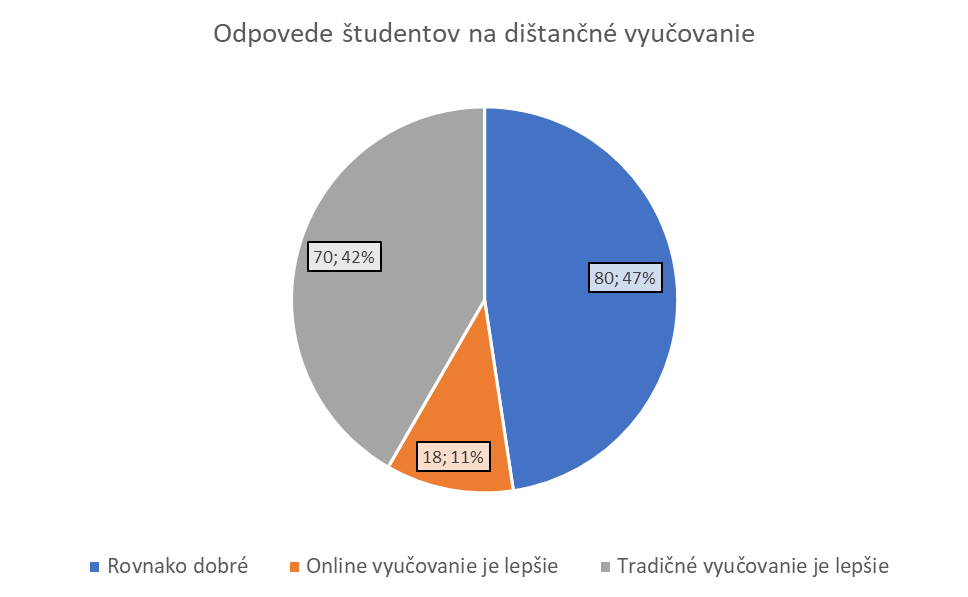
\includegraphics[scale=0.5]{d2.png}
	\caption{Odpovede študentov na efektivitu vyučovania.}
	\label{f:efektivitaStudenti}
\end{figure*}

\begin{table}[]
	\begin{tabular}{|l|l|l|l|l|}
	\hline
	\textbf{Možnosť} &
	  \textbf{\begin{tabular}[c]{@{}l@{}}Počet \\ študentov\end{tabular}} &
	  \textbf{\begin{tabular}[c]{@{}l@{}}\% \\ študentov\end{tabular}} &
	  \textbf{\begin{tabular}[c]{@{}l@{}}Počet \\ učiteľov\end{tabular}} &
	  \textbf{\begin{tabular}[c]{@{}l@{}}\% \\ učiteľov\end{tabular}} \\ \hline
	Obtiažnosť je rovnaká         & 68  & 40,48  & 4  & 36,36  \\ \hline
	Online vyučovanie je ťažšie   & 84  & 50,00  & 5  & 45,45  \\ \hline
	Klasické vyučovanie je ťažšie & 16  & 9,52   & 2  & 18,18  \\ \hline
	Spolu                         & 168 & 100,00 & 11 & 100,00 \\ \hline
	\end{tabular}
	\caption{Odpovede študentov a učiteľov na náročnosť dištančného vyučovania}
	\label{tab:narocnostStudentiUcitelia}
	\end{table}

\subsection{Porovnanie výsledkov}
V roku 2014 bola vykonaná štúdia na viac ako 40 tisíc vysokoškolských študentoch pre porovnanie výsledkov prezenčného vyučovania a dištančného vyučovania. Bolo zistené, že všetci študenti mali horšie výsledky počas dištančného vyučovania. Zároveň sa zistilo, že ľudia s menšími akademickými možnosťami a zručnosťou mali väčšiu pravdepodobnosť, že budú viac negatívne ovplyvnení dištančným vzdelávaním ako ostatní\cite{Zimmerman:Experiment}.

\section{Dopad dištančného vzdelávanie na tradičný spôsob} \label{dopad}
Už teraz je jasné, že aj keď dištančné vzdelávanie nemusí byť tak efektívne ako by sme očakávali alebo chceli, rozhodne ovplyvní tradičné vzdelávanie. Najpravdepobnejší prípad bude, že sa bude uskutočňovať kombinácia oboch spôsobov, a teda pôjde o kombinovanú výučbu (alebo aj \textit{hybridnú výučbu}) - niektoré školy už prestúpili na tento spôsob kvôli pandémii Covid-19\cite{Zimmerman:Experiment}\cite{Ahmed:Model}.

Ďalším pravdepodobným prípadom je, že dištančné vyučovanie pômože pri informatizácii prezenčného vyučovania. Nakúpené zariadenia pre dištančné vyučovanie môžu byť využité aj v prezenčnom vyučovaní, a teda učitelia a žiaci by mohli využívať technológie viac ako doteraz.

\section{Záver} \label{zaver}
Moderná technológia dnešnej doby nám dovolila vykonávať vyučovanie diaľkovo a relatívne jednoducho, avšak na úkor efektivity vzdelávania. Navyše, pandémia ochorenia Covid-19 spustila revolúciu v oblasti školstva, kedy boli školi nútene prejsť na tento spôsob vyučovania a tiež nakúpiť potrebnú technológiu.

Osobne vnímam dištančné vzdelávanie ako alternatívny spôsob vyučovania, ale nepovedal by som, že by mal byť ako primárny. Ak sa pridá fakt, že sa výlučne dištančné vyučovanie využíva dlho, môže to mať rozsiahle negatívne následky na výsledky študentov a študentov samotných.

\paragraph{Spoločenské súvislosti}
Pri dištančnom vyučovaní chýba taký fyzický kontakt medzi ľuďmi ako pri prezenčnom, ľudia si sú vzdialenejší. V niektorých prípadoch sa spolužiaci navzájom ani nepoznajú, čo je v prostredí strednej školy nevídané. Prípadne nepoznajú ani meno učiteľa. Spoločenský kontakt je teda značne obmedzený a najväčšie škody napácha v prostredí nového kolektívu.

\paragraph{Historické súvislosti}
Aj keď to môže znieť prekvapivo, dištančné vyučovanie nie je novinkou. Už v 18. storočí sa isté spôsoby dištančného vzdelávania uskutočňovali, vtedy pomocou poštovej služby. Študentky boli vtedy prevažne ženy, ktoré boli doma kvôli konvencii vtedajšej doby. Neskôr sa používalo rádio, ktoré školy využívali a vysielali prednášky. Postupom času sa začala používať televízia. V dnešnej dobe využívame hlavne počítač a internet. Počas vývoja ľudstva sme teda svedkami výmeny rôznych technológií sprostredkúvajúce šírenie vzdelania\cite{Harting:History}.

\paragraph{Technológia a ľudia}
S vývojom technológií sa dištančné vyučovanie mohlo začať využívať viac a jednoduchšie ako kedykoľvek predtým. Avšak, ako tomu bolo v minulosti, napríklad čo sa rádia týka, muselo byť k dispozícii a človek s ním musel vedieť narábať. Síce nám technológie uľahčujú prístup a komunikáciu, avšak človek si ho musí zadovážiť (čo môže byť problém v sociálne slabších rodinách) a musí s ním vedieť robiť (starší ľudia majú prevažne častejšie problémy pracovať s novými technológiami).

\paragraph{Udržateľnosť a etika}
Udržateľnosť dištančného vyučovania často nie je ideálna, keďže pri dlhodobom dištančnom vyučovaní začína byť negatívne ovplyvnená psychika študentov a sociálny kontakt je obmedzený. Čo sa týka masových online otvorených kurzov (\textit{MOOC}), podstatne menej študentov dokončí takýto typ kurzu ako pri tradičnom spôsobe\cite{Pursel:MOOC}.

\bibliography{literatura}
\bibliographystyle{plain}
\end{document}
